\chapter{Analysis 1: Textual Analysis of GM Seed Discourse}
\lhead{\textit{Analysis 1: Textual Analysis of GM Seed Discourse}}

\textit{\textbf{Chapter Summary}: In this chapter, multilevel analysis is applied to a web-based corpus to examine debates related to genetically modified (GM) seed. Keyword analysis, concordance lines, and collocation are used to explore whether sides in the debate are reflected in the semantic structure of the text. Implicature and conceptual blending point to differences at the cognitive level. Results highlight how misunderstandings can emerge from differing epistemologies, worldviews, and situated contexts.}
\newline

Since its emergence on world markets in the 1990s, genetically modified (GM) food has been a source of controversy and disagreement. The disagreements involve a range of actors including consumers, farmers, multinational companies, regulators, non-governmental organizations, and scientists. Here, we use multilevel analysis to gain an understanding of opposing views on the subject of GM seed. Using corpus-based data and analysis, we contrast perspectives on the issue in order to identify sources of divergence. 	

The GMO debate often focuses on whether or not GM food is safe for human consumption. On the surface, the debate strictly concerns scientific evidence. However, even at the scientific-level, there is much variation in how statements and evidence can be interpreted. For instance, people might respond differently to the claim that there is no evidence of adverse health impacts. Moreover, how people respond to this claim may be influenced by culture, since ``no evidence'' indicates a degree of unpredictability or uncertainty. It is well established that uncertainty avoidance is culturally variable \citep{McCornack2017}.

In addition to debates concerning the science, there are many other aspects to the topic of GM seed. Practices relating to the production and consumption of food go to the core of many cultures and value systems. In addition, production and consumption of food is the basis of economic livelihoods and well-being. Given the many scientific, cultural, and economic dimensions of the topic, it is appropriate to approach GM seed debates through multilevel analysis. 

\section{Corpus Data}

The first corpus contains textual data related to the theme of GM seed. The aim for corpus construction was comparative analysis of two sides of the debate surrounding GM seed (i.e. pro and anti). Thus, the corpus was split into two sub-corpora representing anti- and pro-GM seed perspectives,3 respectively. 

Two sub-corpora were constructed using text from web pages. Web pages were queried and identified manually using the Google search engine with search terms related to GM seed. Some search terms were generic so as to capture perspectives from both sides of the debate (i.e. ``gm seed'', ``gm seed AND seed saving'', ``gm seed debate''). Other search terms were targeted towards a specific side of the debate (i.e. ``gm seed resistance'', ``gm seed opposition'', ``gm seed advantages'', ``gm seed benefits''). Finally, another generic search was included to identify cultural dimensions (``gm seed AND culture'').

For each search, pages were qualitatively identified as representing either an anti- or pro- stance on GM seed. Pages that were ambiguous or were of a `pros and cons' nature were omitted from further consideration, though it was noted that the vast majority were easily identifiable as pro- or con-. For those pages which did take a clear stand on the topic, the associated urls were collected and listed as either anti- or pro-GM seed. About 100 urls for each category were collected in this way. Both categories included pages from ngos, foundations, news agencies, social media, and academic institutions. As might be expected, the pro-GM category included more pages from corporations while the anti- category included more ngos and advocacy groups. Genres included news articles, op eds, blogs, academic articles, reference material, interviews, transcripts, and reports. Another important genre was advocacy statements for organizations.

Once urls were collected, the text from the associated webpages was extracted with a custom script written in the Python language. All texts were agglomerated into one file, such that there were two files, one for the anti- and one pro- corpus.\footnote{The files \textit{anti\_gm.txt} and \textit{pro\_gm.txt} are available in the GitHub repository (link provided in Appendix 1).} Each of the files was then cleaned to remove html tags and other unnecessary syntax. The result was two data files, each a corpus of texts from about 100 sources. After some initial noise removal (removal of punctuation, digits, and special characters), the size of the anti-gmo subcorpus was about 225,000 words while the size of the pro- subcorpus was about 163,000 words. 

To facilitate computational analysis, further pre-processing was done on both data sets using the Natural Language Toolkit (NLTK) Python package. Normalization of the data was done through stemming, lemmatization, and removal of stop words. After this normalization, the size of the anti-gmo subcorpus was about 135,000 words while the size of the pro- subcorpus was about 101,000 words. 

In what follows, the corpus is analyzed in order to shed light on various levels of the GM debate. Linguistic data are compared and contrasted from the two sub-corpora, representing pro- and anti-GM perspectives. Through the data, we seek to determine whether there are quantitative differences between the sub-corpora and, if so, how these differences can be qualitatively explained. For this, corpus methods are combined with discourse analysis. Employing quantitative analysis of large data sets in this way allows for insights that would otherwise not be discernible though manual reading of texts.

\section{Overview of the Data}

An overview of the corpus data provides possible directions for further analysis. This overview is obtained in two ways: first, by considering differences in the sources or the data for the two sub-corpora; second, by comparing keywords and key terms between the two sub-corpora.    

\subsection{Top-level Domains}

Differences in sources of the data refers to where/who the data originate from. As explained above, corpus data was collected from webpages. Understanding more about these webpages will help us understand the corpus as a whole. For instance, if a majority of the pro-GM data originated from webpages based in a specific geographic region, then this would be an important point for further consideration. The same would be the case if the majority of pro-GM webpages were from corporate websites. 

For a quick view of the webpage origins, we consider top-level domains (tlds). These are the last part of the web address. For example, in the domain name \textit{www.domain.com}, the top-level domain is \textit{com}. Top-level domains provide clues as to the origins of the data. For instance, the generic tlds such as \textit{com}, \textit{org}, \textit{gov}, \textit{edu} indicate whether the data originated from commercial, organizational, governmental, or educational bodies, respectively. Also, country code tlds such as \textit{fr} (France) or \textit{uk} (United Kingdom), give insight into the country origins of the data.   

To investigate tlds for the corpus, a list was constructed of all domains used in the data collection. Using Python, urls were parsed to determine the distribution of tlds. The pro-GM corpus was constructed from 89 webpages. Of the urls for these pages, 39 (44 percent) had \textit{org} as the tld and 29 (33 percent) had \textit{com}. The remaining tlds (21 total) were \textit{net}, \textit{edu}, \textit{ca}, \textit{uk}, and a handful of other country codes. The pro-GM corpus consisted of 91 urls of which 50 (55 percent) had \textit{com} and 25 (27 percent) had \textit{org} as the tdls. The remainder (16) were \textit{net}, \textit{edu}, \textit{gov}, \textit{ca}, \textit{uk}, and other country codes.

The numbers indicate that the anti-GM data represent a higher percentage of non-governmental or non-corporate organizations (with \textit{org} tlds), while the pro-GM data represent comparatively more corporate organizations (with \textit{com} tlds). As we go deeper into textual analysis, these basic observations about tdls may be helpful in determining sources of different perspectives on the topic of GM seed. A more in-depth look at organizations/people behind the data will be investigated in the multilevel analysis sections. 

\subsection{Keyword Analysis}

A first comparative glance of the sub-corpora can be obtained through keyword lists. Keywords are words typical of a focus corpus vis-\`a-vis a reference corpus. Classifying the top words compared to a reference corpus reveals a range of contrasts and characteristics of the focus corpus \citep{Kilgarriff2012a}. In addition to keywords, key terms (multi-word noun phrases) can be identified. Using the corpus query tool Sketch Engine, keyword and key term lists were obtained for both sub-corpora. Top words and terms were identified according to a score given by: 

\[ \frac{f_\mathrm{focus}+n}{f_\mathrm{ref}+n} \]

Where \(f_\mathrm{focus}\) is the frequency (per million) in the focus corpus and \(f_\mathrm{ref}\) the frequency in the reference corpus and \(n\) is a smoothing parameter (default \(n=1\)) \citep{Kilgarriff2014a}. The reference corpus was Sketch Engine's web corpus \textit{enTenTen: Corpus of the English Web}.	 

Keyword and key term lists provide an overview of the corpora and indicate possible avenues for further analysis. Below, Table 3.1 shows the top 20 keywords and Table 3.2 shows the top 10 (bi-gram) key terms along with the scores and focus frequencies for both the anti- and pro-GMO sub-corpora. 

\begin{table}[H]
\begin{footnotesize}
\centering
\def\arraystretch{1.1}%
\begin{tabular}{llllll}
\hline
\multicolumn{3}{c}{\textbf{Anti-GMO}}    & \multicolumn{3}{c}{\textbf{Pro-GMO}}   \\
\hline
\textbf{Word}        & \textbf{Score}  & \textbf{Freq.} & \textbf{Word}        & \textbf{Score}   & \textbf{Freq.} \\
\hline
monsanto    & 816.94 & 619   & ht          & 1710.97 & 665   \\
gmos        & 791.46 & 353   & eiq         & 1394.56 & 291   \\
peoples     & 642.26 & 554   & herbicide   & 857.48  & 591   \\
maize       & 576.19 & 379   & gm          & 768.84  & 1926  \\
gmo         & 477.85 & 324   & maize       & 757.65  & 395   \\
soya        & 352.18 & 151   & tillage     & 688.04  & 202   \\
biocultural & 321.83 & 85    & soybean     & 683.11  & 613   \\
indigenous  & 304.84 & 1097  & insecticide & 512.21  & 312   \\
herbicide   & 301.44 & 262   & ha          & 484.71  & 1114  \\
gm          & 297.41 & 940   & glyphosate  & 468.27  & 138   \\
bt          & 292.49 & 146   & bt          & 442.13  & 175   \\
transgenic  & 285.48 & 119   & ir          & 430.18  & 335   \\
genetically & 281.36 & 415   & monsanto    & 416.52  & 250   \\
biocultural & 244.12 & 66    & biotech     & 414.95  & 234   \\
sovereignty & 207.72 & 55    & crops       & 407.03  & 103   \\
roundup     & 200.43 & 94    & canola      & 390.11  & 179   \\
glyphosate  & 194.02 & 72    & gmos        & 331.37  & 117  
\end{tabular}
\caption{Keywords from the sub-corpora (ranked by score).}
\label{tab:table1}
\end{footnotesize}
\end{table}

\begin{table}[H]
\begin{footnotesize}
\centering
\def\arraystretch{1.1}%
\begin{tabular}{llllll}
\hline
\multicolumn{3}{c}{\textbf{Anti-GMO}}    & \multicolumn{3}{c}{\textbf{Pro-GMO}}   \\
\hline
\textbf{Word}        & \textbf{Score}  & \textbf{Freq.} & \textbf{Word}        & \textbf{Score}   & \textbf{Freq.} \\
\hline
food sovereignty & 406.57 & 126   & farm income & 1107.66 & 251   \\
traditional food & 300.48 & 94    & crop impact & 949.56  & 197   \\
bt maize & 218.5  & 57 & farm level & 456.68  & 99    \\
traditional knowledge & 218.43 & 82 & soil carbon & 391.81  & 88    \\
oilseed rape & 196.6  & 61 & carbon sequestration & 376.53  & 102   \\
biocultural diversity & 167.53 & 49 & bt cotton & 359.88  & 77    \\
seed market & 129.7 & 34 & income gain & 342.87  & 71    \\
genetic diversity & 125.82 & 46 & income impact & 331.91  & 69    \\
genetic engineering & 121.19 & 51 & weed control & 324.33  & 85    \\
seed sovereignty & 110.33 & 29 & herbicide use & 317.93  & 68   
\end{tabular}
\caption{Key terms from the sub-corpora (ranked by score).}
\label{tab:table1}
\end{footnotesize}
\end{table}

There are several keyword differences between the two sub-corpora. The anti-GMO subcorpus contains a higher incidence of culturally significant words and terms, notably \textit{peoples}, \textit{biocultural}, \textit{indigenous}, \textit{sovereignty}, \textit{traditional food}, \textit{traditional knowledge}, and \textit{biocultural diversity}. What these items suggest is that the anti-GM discourse is embedded in a context of group identities, traditions, and intersubjective meanings. In addition to the scientific and technical terminology (e.g., \textit{transgenic}, \textit{glyphosate}, \textit{Bt}), the cultural and social aspects are present in a way that they are not in the pro-GM data. 

By contrast, the pro-GM subcorpus features more technical and specialized words and terms. There are higher frequencies of abbreviations like \textit{ht} (herbicide tolerant), \textit{eiq} (environmental impact quotient), and \textit{ir} (insect resistant). The use of abbreviations suggests more dense technical discourse. The key terms list also features several items related to income, indicating that economic gain and efficiency is a more prevalent theme in the pro-GM corpus. 

Similar conclusions can be drawn by looking at the top n-grams (sequences of \textit{n} words). These were determined by taking the top frequencies on an absolute basis (i.e. not using a reference corpus for comparison). After removing stop words, the 20 most frequent uni-grams, bi-grams, and tri-grams (1-, 2-, and 3-word sequences) were determined for each corpus.

As expected, there are several top keywords common to both sub-corpora such as \textit{gm} and \textit{genetically modified}. However, there are also notable differences. For instance, in the top-20 lists obtained from the anti-GM corpus, the following n-grams are present:

\begin{quote}
\textit{indigenous}, \textit{people}, \textit{traditional}, \textit{cultural}, \textit{community}, \textit{food sovereignty}, \textit{biocultural diversity}, \textit{traditional knowledge}, \textit{agro ecological system}, \textit{right indigenous people}, \textit{sovereignty}, \textit{critical dialogue}.   
\end{quote}

These n-grams are indicative of a certain cultural as well as socio-economic context rooted in identity, tradition, and food sovereignty. By contrast, the pro-GM corpus features more abbreviations as well as technical language related to agrochemicals and agribusiness. For example, the pro-GM corpus contains the following n-grams in the top-20 lists:

\begin{quote}
\textit{ht}, \textit{herbacide}, \textit{cotton}, \textit{cost}, \textit{yeild}, \textit{gm ht}, \textit{gm ir}, \textit{farm income}, \textit{ht soybean}, \textit{yeild}, \textit{cost saving}, \textit{biotech crop}, \textit{farm income gain}, \textit{kg carbon ha}, \textit{income impact using}. 
\end{quote}

A preliminary view of the corpus suggests multiple discursive themes are present in the corpus. In addition to ecological/scientific aspects, culture seems to be a major factor in the anti-GM corpus. Also, the presence of economic terms suggests that socio-economic factors are also central, with \textit{income} and related terms featured more in the pro-GM corpus. Also, the pro-GM corpus seems to contain more abbreviations and terminology related to agrochemicals/agribusiness. 

As with the preceding data on top-level domains, these are only precursory observations and further analysis is needed before drawing any conclusions. 

\section{Multilevel Analysis}

The initial overview of the data suggests possible avenues by which to understand the GM seed debate. In particular, the keyword analysis confirms that the topic of GM seed touches on a complex interplay of scientific, cultural, and economic dimensions. Moreover, the data suggest that these dimensions differ between the between pro- and anti- perspectives.

The sections that follow look at each level separately, expanding on themes that emerged in the overview of the data.

\subsection{Ecological Level}

Chapter 2 introduced the ecological-level of discourse. This level asks us to consider the ecological context of language and communication. Simply put, the premise is that the way in which humans speak and communicate about the natural world matters. Communication about nature reflects deeply held worldviews and beliefs. Communication also constitutes environmentally destructive actions. This section applies the ecological level in the context of GM seed discourse. The corpus provides discourse surrounding GM seeds, allowing us to ask how this discourse reflects certain worldviews, values, and beliefs.  

GM seeds are those whose DNA has been modified using genetic engineering methods. One might question how something as fundamental as the molecular building blocks of organisms and life, concerns the realm of worldviews and human values. Or, more precisely, one might ask how is it that gene sequences\textemdash which are empirically measured and scientifically understood\textemdash can lead to clashes of worldviews and values. One explanation for diverging perspectives is that there are different, culturally variable, ways of understanding complexity and unpredictability. In the face of this complexity, views on whether and how humans interact with nature's processes (e.g., by altering plant DNA), might be culturally variable.

Ecology\textemdash as the study of how organisms relate to one another and their physical surroundings\textemdash aims to understand interactions from the molecular level all the way to entire organisms, ecosystems, and the planet itself. Ecological interactions give rise to emergent and interdependent complex systems \citep{Bar-Yam2002a}. While the scientific method provides insights into ecological interactions, the complex nature of these interactions may preclude surveyable, reductionist understandings. This unsurveyable characteristic of living systems might manifest as unpredictability. Gene editing and its ecological implications may fall into the realm of what \cite*{Jasanoff2003a} calls ``the unknown, the uncertain, the ambiguous, and the uncontrollable'' (227). 

Ecological complexity might also imply that, in addition to scientific understanding, humans interpret the natural environment semiotically. Chapter 2 posits that humans experience nature as semiosis; that is, nature itself is the source of signs and symbols to which humans ascribe meaning. Rather than third person spectators with an objective, subject-object relationship to nature, humans are embedded in nature and experience it first-hand. Thus, from a standpoint of humanistic inquiry, biological and ecological phenomena can be understood and interpreted metaphorically and symbolically. In other words, natural semiosis carries over into human (cultural) semiosis. Taking gene expression as a type of natural semiosis, discourse in the corpus might reflect how language ascribes meaning to nature, even at its most basic level of DNA. 

To summarize, the human understanding of nature is commonly thought of through universal laws obtained through the scientific method. However, nature is also culturally framed by worldviews (\textit{Weltanschaung}) \citep[217-228]{Dahl2016}. How people understand and communicate about of gene editing technology will depend on worldviews with which they make sense of biological and ecological systems. These worldviews may be heavily influenced by natural science, but also concern complexity, unpredictability, and even the unknown. Of interest in the ecological-level of analysis is whether and how the different sub-corpora reflect different worldviews or ways of understanding nature. 

\textbf{Specialization \& Communities of Practice}

Different understandings of nature can first be approached by looking at how specialized terminology is used in the corpus. Tables 3.1 and 3.2 show that many words appearing in both keyword lists are scientific and technical terms, including \textit{gmo}, \textit{glyphosate}, \textit{herbicide}, and \textit{bt}. These shared terms suggest that, despite diverging perspectives between the two corpora, scientific terminology serves as a common language through both sub-corpora. That said, the keyword list from the pro-GM corpus contains more abbreviations and industry-specific terminology, suggesting more specialized discourse. It is possible that the pro- and anti- perspectives represent different specialized groups or communities of practice which, in turn, employ different assumptions and methods for understanding natural systems.  

To test whether one subcorpus is indeed more technical, lexical diversity can be calculated to determine how the corpora compare with average spoken or written language. One measure of lexical diversity is the type-token ratio (TTR), which is calculated by taking the number of different words in the corpus (word types) and dividing by the total number of words (tokens).

\[ TTR = \frac{Word\:Types}{Word\:Tokens} \]

It has been hypothesized that scientific and technical writing has a lower TTR \citep{Tagliacozza1976a}. The rationale is that technical writings are often more confined in subject matter than more general writings. With precision as the aim of scientific writing, the vocabulary tends to be more limited. The type-token ratio will thus be lower.

Since TTR varies widely based on the number of word tokens, a standardized TTR (STTR) is a better basis for comparison. STTR breaks the corpus into segments (e.g. 2,000 words) and takes the mean TTR over all the segments. Using 2,000 word segments, the STTR was calculated for both sub-corpora. The anti- and pro- GM sub-corpora have ratios of 0.45 and 0.42 respectively. (See Appendix 1 for calculations.) Thus, the anti-GM corpus is more lexically diverse, but not significantly so. By comparison, the FLOB corpus of British English (consisting of written texts from different genres) is 0.45 and that of a spoken segment of the British National Corpus is 0.33, reflecting the more lexically repetitive nature of spoken language \citep[52]{Baker2006b}. 

A more direct measure of the presence of scientific terminology is comparison of the corpora with a dictionary of scientific terms. To conduct such a comparison, a molecular biology glossary was used which comprised of 170 terms \citep{Lyonsa}. The sub-corpora were then tokenized and counts taken for the frequency of glossary terms. To account for the different sizes of corpora, frequencies were based on a random sample of 100,000 tokens from each corpus. The average frequency was then calculated over 100 random samples. The average frequency for anti-GM corpus is 102 per 100,000 while that of the pro-GM corpus is 439. To understand this difference, a dictionary was constructed to determine precisely which molecular biology terms appear in each subcorpus (e.g., {`gene':445}). This shows that \textit{NT} is the most frequent term in the pro-GM corpus. In the glossary, \textit{NT} is an abbreviation for `nucleotide'. However, looking at concordances of \textit{NT} in the corpus, shows that it is an abbreviation for `no-till' agriculture. Removing NT from the glossary results in frequencies that are somewhat closer between the two sub-corpora, but still over twice as high in the pro-GM corpus: the average frequency of anti-GM corpus is 79 and that of the pro- corpus is 206. Therefore, there is evidence to suggest the pro-GM corpus contains more molecular biology terms. However, the dictionary counts show that most molecular biology terms appearing in both corpora are the rather generic \textit{DNA}, \textit{genome}, and \textit{genetic}. These terms are expected given the subject matter and are not necessarily an indication of the level of technicality of either corpus.	

To further assess the level of scientific and technical specialization, the same dictionary process was repeated with a glossary of agrochemicals. Common names of 2,498 herbicides \citep{UniversityofKentuckya} and pesticides \citep{Wood2018a} were collected and frequencies obtained for both sub-corpora. The results indicate the pro-GM corpus has significantly more agrochemical terminology. The pro-GM corpus has an average of 596 per 100,000 words while that of the anti-GM corpus is 92. Moreover, the pro-GM corpus has a greater variety of agrochemicals with 37 (versus 7 in the anti-corpus). This result serves as evidence for the hypothesis that the pro-GM corpus is indeed more scientifically and technically specialized, at least with respect to molecular biology and agrochemical terminology.

If one takes epistemic communities or communities of practice as ``epistemic cultures'' \citep{Knorr-Cetina1999}, then the degree of specialization in certain knowledge areas points to possible sources of misunderstanding between the two sides of the debate. Sources of misunderstanding, therefore, may be attributed to epistemological differences among natural scientific fields of inquiry. Moreover, as \cite*{Reyes-Galindo2017a} point out, science and technology are ``linguistically, epistemically, and socioculturally inaccessible to most members of the wider societies they are immersed in'' (2). Misunderstanding might be attributable to specialized discourses as well as divergent contexts. 

The higher prevalence of agrochemical terms in the pro-GM corpus points to possible epistemic differences but does not, in itself, explain if and how different worldviews are inherent in the corpora. Concordance lines provide a closer view of the data and might point in the direction of deeper cultural differences.

\textbf{Usage of \textit{Ecological} and \textit{Biological}}

Both the keyword and frequency data suggest that the two sub-corpora reflect different epistemological orientations towards the natural world. To investigate this possibility, we can consider concordance or Key Word in Context (KWIC) lines. Specifically, concordances of the words \textit{ecological} and \textit{biological} can provide insight into how living systems are referred to linguistically. 

The anti-GM subcorpus has 107 lines containing \textit{ecological}, compared to only 14 for the pro- subcorpus. These numbers further point to epistemic differences. Whereas the pro-GM corpus is focused more at the molecular level (as indicated by the greater presence of agrochemical terms), the anti-GM corpus seems more concerned with the higher levels of the organization of life and the interrelations between organisms and their environment. Table 3.3 shows a sampling of concordance lines for the anti-GM subcorpus. 

One way to examine how the word \textit{ecological} functions in the corpus is to look at the nouns it modifies. In Table 3.3, nouns modified by the adjective \textit{ecological} include \textit{relationships}, \textit{processes}, \textit{systems}, \textit{complexity}, and \textit{cycles}. In the context of worldviews, these concordances suggest natural phenomena are understood as dynamic interactions, in a holistic sense. By contrast, in the pro-GM concordances in Table 3.4, ecological modifies \textit{farming}, \textit{agriculture}, \textit{component}, and \textit{impacts}. The emphasis on dynamic ecological systems is not as pronounced. Concordances in the pro- corpus suggest more reductive and mechanistic (as opposed to holistic or organicist) approaches to nature.

\begin{table}[h]
\begin{footnotesize}
\centering
\def\arraystretch{1.1}%
 \begin{tabular}{c} 

\texttt{\ myths. While their agro-ECOLOGICAL and food systems offer s } \\ 
\texttt{i cannot sustain further ECOLOGICAL destruction from the imp} \\ 
\texttt{ncrease biodiversity and ECOLOGICAL resilience, and contribu} \\ 
\texttt{e of plants, animals and ECOLOGICAL processes," added the IP} \\ 
\texttt{nsecticidal toxicity to ECOLOGICAL complexity'', BioScience} \\ 
\texttt{wledge of local species, ECOLOGICAL relationships, and ecosy} \\ 
\texttt{\ \ practices to suit their \ ECOLOGICAL niches. This meant learn } \\ 
\texttt{out plants, animals, and ECOLOGICAL processes, as well as sp} \\ 
\texttt{interpreting social and ECOLOGICAL systems, as well as the  }\\ 
\texttt{ from nutrient cycles to ECOLOGICAL niches, from interand in} \\ 
\texttt{ governance. social and ECOLOGICAL systems and achieving th} \\ 
\texttt{ tional trade and natural ECOLOGICAL cycles. While exploring } \\ 
\texttt{e of plants, animals and ECOLOGICAL processes," added the IP} \\
 \end{tabular}
\caption{Concordance lines of \textit{ecological} Anti-GM corpus}
\label{tab:table1}
\end{footnotesize}
\end{table}

\begin{table}[h]
\begin{footnotesize}
\centering
\def\arraystretch{1.1}%
 \begin{tabular}{c} 

\texttt{\ \ combined with a volatile ECOLOGICAL climate and socioeconomi} \\ 
\texttt{\ \ \ This is one of the many ECOLOGICAL farming practices he use} \\ 
\texttt{\ \ \ with real food based on ECOLOGICAL agriculture not only add} \\ 
\texttt{\ \ ing in climate-resilient ECOLOGICAL agriculture and empoweri} \\ 
\texttt{\ eets, describing health, ECOLOGICAL, and environmental effe} \\ 
\texttt{\ \ \ nsumer component, and an ECOLOGICAL component. Each componen} \\ 
\texttt{\ \ \ rm worker, consumer, and ECOLOGICAL components: EIQ=\{C[(DT*5} \\ 
\texttt{\ absorbed by plants). The ECOLOGICAL component of the model i} \\ 
\texttt{\  rm worker, consumer, and ECOLOGICAL) and the average EIQ va} \\ 
\texttt{\ \ sessing the economic and ECOLOGICAL impacts of herbicide tol} \\ 
 \end{tabular}
\caption{Concordance lines of \textit{ecological} Pro-GM corpus}
\label{tab:table1}
\end{footnotesize}
\end{table}

Repeating the analysis on concordances of \textit{biological} gives similar results. Again, the anti-GM corpus contains a higher frequency of \textit{biological} concordance lines (94 versus 10). Nearly half of all concordances in the anti-GM subcorpus contain the collocate \textit{biological diversity}. As Table 3.5 shows, other nouns modified include \textit{evolution}, \textit{balance}, \textit{processes}, and \textit{hotspot}. As with the ecological concordances, the word \textit{biological} is used to describe complex and holistic systems. Table 3.6 shows nouns in the pro-GM concordances including \textit{resource}, \textit{solution}, \textit{methods}, \textit{screening}, and \textit{controls}. Again, the notion that life processes are manageable, reducible, and analyzable suggests a different epistemological orientation to nature than is apparent in the anti-GM corpus.

\begin{table}[h]
\begin{footnotesize}
\centering
\def\arraystretch{1.1}%
 \begin{tabular}{c} 

\texttt{, sometimes cultural and BIOLOGICAL diversity are correlated} \\ 
\texttt{ins millions of years of BIOLOGICAL and cultural evolution o} \\ 
\texttt{ substantial risk to the BIOLOGICAL balance of nature", Lerc} \\ 
\texttt{rmers, the threat to the BIOLOGICAL diversity of corn, the c} \\ 
\texttt{s to be based on natural BIOLOGICAL processes and a precauti} \\ 
\texttt{\ \ \ \ afety means that the BIOLOGICAL diversity of crops is de} \\ 
\texttt{\ Grosso's territory is a BIOLOGICAL hotspot with over 55,000} \\ 
 \end{tabular}
\caption{Concordance lines of \textit{biological} Anti-GM corpus}
\label{tab:table1}
\end{footnotesize}
\end{table}

\begin{table}[h]
\begin{footnotesize}
\centering
\def\arraystretch{1.1}%
 \begin{tabular}{c} 
\texttt{\ nable modification of a BIOLOGICAL resource--is going to be} \\ 
\texttt{\ \ in arguing the need for BIOLOGICAL solutions, like GM, to r} \\ 
\texttt{n and expand research in BIOLOGICAL science-based programs.} \\ 
\texttt{\ \ \ innovative chemical and BIOLOGICAL solutions. Aligning thes} \\ 
\texttt{\ \ automated synthesis and BIOLOGICAL methods to prepare the q} \\ 
\texttt{\ \ ds required for targeted BIOLOGICAL screening. We use a stru} \\ 
\texttt{\ \ the plant metabolism or BIOLOGICAL activity, through to the} \\ 
\texttt{rmers (e.g. new types of BIOLOGICAL controls) are tested for} \\ 
\texttt{\ \ of alternatives such as BIOLOGICAL and cultural control mea} \\ 
\texttt{\ n of the data on diverse BIOLOGICAL and societal aspects of } \\ 
\texttt{\ udies that found adverse BIOLOGICAL or social effects of GE } \\ 
 \end{tabular}
\caption{Concordance lines of \textit{biological} Pro-GM corpus}
\label{tab:table1}
\end{footnotesize}
\end{table}

\textbf{Summary of the Ecological-level}

Through the preceding ecological-level analyses we can begin to see possible sources of misunderstanding between the two sides of the GM seed debate. The data suggest that natural science (specifically molecular biology) is a common language across both sides of the debate. However, the extent of this common language is limited, since the pro-GM subcorpus contains a higher frequency of molecular biology terminology. There is also evidence that the pro-GM corpus contains a much higher frequency of agrochemical terms. This result suggests that the pro- side of the debate is representative of more specialized communities of practice dealing with chemical/agrochemical technologies. Accordingly, one might consider sources of misunderstanding as being rooted in different disciplinary assumptions and epistemic presuppositions. 

Concordance analysis takes epistemic differences a step further and points to different approaches to understanding the natural world. What emerges is, in the anti-GM subcorpus, a organicist and holistic approach and, in the other, analytic and mechanistic approaches. The question of whether these differences are indicative of entire worldviews (and hence cultures) can be further examined in the cultural-level of analysis.       

\subsection{Cultural Level}

\textbf{Concordances of \textit{Culture}}

To consider the cultural context, we can begin by looking at how the word \textit{culture} is used in context within and between the sub-corpora. Concordances of the word \textit{culture} give insight into this context as well as the meanings of the term within the corpus. There are 215 mentions of \textit{culture} in the corpus as a whole. Nearly all (211) of these mentions are in the anti-GM subcorpus, further indicating what the keywords analysis suggests; namely, that anti-GM discourse is embedded in a cultural context in a way that pro-GM discourse is not. Furthermore, 3 of the 4 mentions of culture in the pro-GM subcorpus use \textit{culture} as a biological term (e.g., \textit{tissue culture}).

Table 3.7 shows a sample of concordances from the anti-GM subcorpus. A qualitative assessment of the concordance lines indicates how culture stands in relation to other discourse themes and, ultimately, to the overall theme of seed. For example, the close relation between food and culture stands out in lines such as ``...food as part of culture and identity''; ``Culture without food is not culture''; and ``...unique food systems and culture.'' These associations indicate that anti-GM discourse views seed in relation to food production, consumption, and cultural identity. Generally, the concordance lines point to culture as something valuable to be preserved. Collocated words like \textit{customs}, \textit{traditional}, \textit{ancient}, and \textit{preserve} are all indicative of the idea of culture as something of deep meaning and value. While most uses of `culture' are positive or affirming, it is also used in a pejorative sense. For instance, phrases ``consumer culture,'' ``capitalistic culture,'' and ``today's culture'' indicate that modern culture is held in critical view. Thus, a juxtaposition of cultures is at play in the discourse.

\begin{table}[h]
\begin{footnotesize}
\centering
\def\arraystretch{1.1}%
 \begin{tabular}{c} 
\texttt{that are rare in today's CULTURE. Seed saving, once an es} \\
\texttt{ntral to our being, our CULTURE and our relationship to} \\
\texttt{ us; for any sustainable CULTURE has its roots in the lan} \\
\texttt{e the bearer of life and CULTURE, yet most of today's com} \\
\texttt{ time immemorial and our CULTURE, myths, dreaming and sac} \\
\texttt{ unique food systems and CULTURE. Indigenous women are al} \\
\texttt{and agriculturally savvy CULTURE has won a major battle a} \\
\texttt{hunting and food-sharing CULTURE, as reduced sea ice caus} \\
\texttt{nd movement. And as our CULTURE, again, as I say, is bas} \\
\texttt{ the foundations of our CULTURE, to safeguard our river} \\ 
\texttt{ance with our health and CULTURE. Re-establishing ancient} \\
\texttt{e strive to maintain our CULTURE and resist the global, i} \\
\texttt{learning the science and CULTURE of their ancient corn, i} \\
\texttt{corn to the identity and CULTURE of Mexicans, and the cor} \\
\texttt{ry important part of our CULTURE. The pyramids may have b} \\
\texttt{ unique food systems and CULTURE. Indigenous women are al} \\
\texttt{\ al links with indigenous CULTURE and food sovereignty. La} \\
\texttt{curity, livelihoods and CULTURE of farming communities.} \\ 
\texttt{hin the context of their CULTURE. I read it as an ancestr} \\
\texttt{eed is the embodiment of CULTURE because culture shaped t} \\
\texttt{\ such an outrage. Every CULTURE that I've come across be} \\
\texttt{merican Indians to their CULTURE and renew interest in he} \\
\texttt{r relationship to place, CULTURE, plants, and all of natu} \\
\texttt{ of seed savers and seed CULTURE keepers in the United St} \\
\texttt{\ \ ash, tobacco, and Din\'e CULTURE: ``It's part of reclaimin} \\
\texttt{ place its heritage, its CULTURE and a palpable expressio} \\
\texttt{ and as the mandala of a CULTURE. Honoring a time-old tra} \\
\texttt{ps, preserve history and CULTURE, promote bio-diversity a} \\
\texttt{. From this seed saving CULTURE birthed some of our favo} \\
\texttt{ntral to our being, our CULTURE and our relationship to} \\
\texttt{t us to our history, our CULTURE, our family, and our sen} \\
\texttt{ static image of relict CULTURE. Traditional ecological} \\ 

 \end{tabular}
\caption{Concordance lines of \textit{culture} Anti-GM corpus}
\label{tab:table1}
\end{footnotesize}
\end{table}

Both keywords and concordances point to the interrelations between ecology and culture. The tradition of seed saving is thousands of years old and traces back to the origins of agriculture and even human society itself. In modern times, however, the use of commercially patented and owned seed often precludes or prohibits collecting, saving, planting, harvesting, and exchanging seed.

Viewing seed discourse in ethnographic terms reveals rich symbolic associations between ecology and culture. Through linguistic utterances, we see how natural and biological processes work as connotations for how people understand themselves as living beings that are parts of a holistic natural order. By contrast, much GM discourse frames the topic in more literal or denotative terms. Based on this observation, it is conceivable that disagreements concerning GM seed stem from a failure to acknowledge cultural associations and connotations. 

Table 3.7 suggests that the cultural concept of \textit{indigenous} is prominent in the corpus. To see how this concept is split between the sub-corpora, frequencies of \textit{indigenous} were calculated for each. The anti-GM corpus has 784 unique mentions of the work \textit{indigenous} while the pro-corpus has none. This result is further indicative of a vastly different cultural context between the anti and pro corpora. 

The concordances in Table 3.7 give an idea of how \textit{culture}, in a general sense, functions in the corpus. However, the lines say little about which cultures are represented. To gain a better idea of different cultures in the corpus, we can consider geographic entities.  

\textbf{Distribution of Geographic Entities}

One way to understand cultural variation, is to consider the distribution of geographic entities in the corpus data. In other words, we can consider how different national/cultural regions are represented in segments of the data. Specifically, we can extract and analyze city and country names as a proxy for possible cultural variation. 

There are a number of reasons for investigating geographic distribution in this way. For instance, investigating geographic origins of the data might reveal bias. The corpus data was collected using commercial search engines, which have been shown to be have bias towards websites from certain countries. Previous visits to a site and the number of links to it affects its chance of appearing in search engine results \citep{Vaughan2013a}. Corpus data might also reflect how perspectives in the GM-seed debate diverge along national lines. Some argue that that small-scale farmers in the Global South are the losers in the shift toward GM seed, while corporations and farmers in the Global North are those who benefit \citep{Parfitt2013a, Nu2009a}. Accordingly, one might expect the pro- and anti-GM sub-corpora to reflect more Global North and Global South sources, respectively.

As one might expect, a preliminary overview of the urls and organizations from which data was collected suggests that data originate from companies, NGOs, and media agencies based in North America or Western Europe. This was the case for both sub-corpora. However, this does not mean other parts of the world are not in the data. The frequency of country names (i.e. the total number of mentions of any country name), shows that many country names are not North American or European. To further pursue this line of investigation, some entity extraction and quantitative analysis is necessary. 

Using the Python software package geotext \citep{Palenzuelaa} country names were extracted from each subcorpus. Initially, this way of extracting only the countries mentioned in the corpora revealed some limitations in this method. High frequencies are observed for Canada, which may be due to the fact that corpus data was collected from a Canadian-based IP address, so Canadian websites (e.g., news reports) might have ranked higher on search results. Also, there is an absence of the United States from top-5 countries despite the fact that, based on a qualitative scan of the data, much of the data reference US institutions and locations. This absence points to another possible limitation of using frequencies of country names alone. It is common to reference geographic locations through cities or states rather than counties, particularly if these locations are well-known or familiar to the audience. For instance, in the line ``anthropologist and associate professor at Dalhousie University in Halifax, Canada'' it is necessary to reference ``Canada'' whereas in the line ``The lawsuit, filed on behalf of farmers by the Washington, D.C., law firm,'' a reference to the United States would be redundant. The net effect is an under representation of geographic entities containing large, well-known cities.

To account for this limitation in country frequencies, a similar entity recognition method was also used to account for city names. City names were identified in each supcorpus using \textit{geotext}. Using a database of world cities, the city names were filtered to limit those with a population of at least 500,000. The corresponding countries were then counted and added to the country counts. Table 3.8 gives the top-10 countries in each subcorpus ranked by frequency (per 1,000 words). This method places the United States and Canada clearly at or near the top of both sub-corpora. Moreover, using the cities method, the frequencies are generally higher in the pro-GM corpus. For example, the tenth country on the pro-GM list (Philippines) has a higher frequency (0.29) than the sixth country on the anti-GM list (Nepal). This suggests that urban centers (with population greater than 500,000) are more frequently mentioned in the pro-GM subcorpus. 

\begin{table}[h]
\begin{footnotesize}
\centering
\begin{tabular}{|l|l|l|l|}
\hline
\multicolumn{2}{|l|}{\textbf{Anti-GM Corpus}} & \multicolumn{2}{l|}{\textbf{Pro-GM Corpus}} \\ \hline
\textbf{Country}       & \textbf{Freq.}       & \textbf{Country}      & \textbf{Freq.}      \\ \hline
Mexico                 & 0.82                  & Canada         & 1.04                \\ \hline
United States          & 0.70                 & Argentina                & 0.91               \\ \hline
Canada                 & 0.45                 & United States                & 0.77                \\ \hline
India                  & 0.39                 & Brazil             & 0.67                 \\ \hline
Colombia               & 0.30                 & India                 & 0.60                 \\ \hline
Nepal                  & 0.28                 & Australia                & 0.39                \\ \hline
Argentina              & 0.27                 & South Africa              & 0.38                 \\ \hline
Haiti                  & 0.25                 & Mexico             & 0.34                \\ \hline
Brazil                 & 0.20                 & China          & 0.32                \\ \hline
Guatemala              & 0.17                 & Philippines                 & 0.29                \\ \hline
\end{tabular}
\caption{Geographic entities summary}
\label{tab:table1}
\end{footnotesize}
\end{table}

Most countries are overlapping between both sub-corpora (i.e. US, Canada, Mexico, India, Argentina, and Brazil). However, of interest are the outliers. In the anti-GM corpus, these outliers are Nepal, Haiti, Colombia, and Guatemala. In the pro-GM corpus they are Australia, South Africa, and China, and Philippines. Generally speaking, the outliers in the anti-corpus are smaller economies and less-developed countries. This lends credence to the suggestion that the anti-corpus might reflect more perspectives from the Global South or the more economically disenfranchised. To test this hypothesis, the package \textit{country converter} \citep{Stadler2014} was used to classify all countries in the corpus (including those derived from city mentions) according to the United Nations geoscheme. From this, the total number of country-mentions from ``Global North'' and ``Global South'' was determined. The anti-GM corpus has 38 percent of countries from the Global South while the pro-GM corpus has only 13 percent. So, both sub-corpora have the majority in the Global North, with the pro-GM corpus having a significantly higher percentage of country mentions from the Global North. This finding will be discussed at greater length in the subsequent section, the \textit{Socio-Economic Level}.

Table 3.8 shows only the top 10 of 92 countries in the corpus. The distribution of the remaining countries can also say much about cultures in the corpus. To understand the geographic entities as a whole, we look to the diversity of the country data, or the extent to which country data are concentrated (with a few countries mentioned frequently) or distributed (with many countries mentioned less frequently). To measure the distribution of country frequencies across the entire data set, we can use concepts from information theory \citep{Shannon1949}; namely, Shannon's diversity index, \(H\), and Shannon's equitability, \(E_H\), which are calculated as follows:

$$H=-\sum_{n=1}^{S} p_i ln p_i$$

$$E_H=\frac{H}{\ln{S}}$$

where \(S\) is the total number of items in the dataset, \(p_i\) is the proportion of \(S\) belonging to the \(i^{th}\) member of the dataset. \textit{Shannon's diversity index} is used to measure the uncertainty or entropy of data and is a popular method to measure diversity of, for instance, ecological systems. Equitability computes a value between 0 and 1, with 1 being complete evenness. In the present analysis, we are interested in diversity of the country/frequency data; that is, the distribution of frequencies across different countries, with \(p_i\) being the proportion of all frequencies attributed to a given country \(i\).

\textit{Shannon's diversity index}, \(H\) was calculated for both sub-corpora. Calculating with the frequency data, results in \(H=2.61\) for the anti-GM corpus and \(H=1.3\) for the pro-corpus. \textit{Shannon's equitability}, \(E_H\) was then calculated. Each dataset was normalized using \(S=195\) as the total number of possible countries. Calculation results in \(E_H=0.49\) for the anti-GM corpus and \(E_H=0.25\) for the pro-corpus. In other words, the diversity and evenness of country frequencies is about twice as high in the anti-GM data. This suggests that the anti-corpus contains a greater variety of countries and, in turn, might reflect a greater diversity of cultural perspectives.

\textbf{Temporal Horizons \& Historical Context}

Cultural dimensions can also be explored through the historical and temporal context of the corpus. Cultural memory is inter-generational and historical. Therefore, based on the premise that the anti-GM corpus is imbued with expressions of cultural identity, one might expect the time span of this subcorpus to be more expansive. A general overview of time span can be obtained through concordances of \textit{century} and \textit{centuries}. These instances were obtained by querying the anti-GM corpus for \textit{centur}* (where * is a wildcard string), which results in 43 lines, 34 of which are in the anti-corpus. The concordances refer to agricultural practices, plant breeding, land tenure through the course of \textit{centuries}. There are also several statements about developments in the 20\textsuperscript{th} century, when the Green Revolution and genetic modification fundamentally altered the practice of food production.  The lines contain references to continents and nations (\textit{Spanish}, \textit{Panama}, \textit{Mexico}, \textit{America}, \textit{Europe}). There are also pronoun references to specific groups, as in the lines: ``\textbf{they} had depended on it for centuries...''; ``seeds from \textbf{their} crops for centuries...''; and, ``During the past five centuries, while \textbf{our} people...''. In such lines, one can see how the temporal horizons connect to back to histories and collective memories of peoples and cultures.
   
The time span of the pro-GM concordances is generally much narrower, with half of the pro-GM concordances falling on \textit{this century} or the \textit{21\textsuperscript{st} century}. Moreover, in the pro-GM subcorpus there are only 2 instances of centuries being used to refer to multiple centuries (i.e. ``\textbf{for} centuries'', ``\textbf{many} centuries''). In the anti-GM subcorpus there are 11 such instances (e.g. ``\textbf{the course of} centuries'', ``\textbf{over} the centuries'', ``\textbf{five} centuries''). Concordances from the anti-corpus data (Table 3.9) suggest that this subcorpus is historically and temporally more expansive.

\begin{table}[H]
\begin{footnotesize}
\centering
\def\arraystretch{1.1}%
 \begin{tabular}{c} 

\texttt{\ \ s have been enriched over the CENTURIES through the abundant biodiver} \\
\texttt{conflict (Spanish in the 16th CENTURY , expropriation of land in th} \\
\texttt{nous economies since the 16th CENTURY , they have retained extensiv} \\
\texttt{\ \ ks, which are the products of CENTURIES of deliberate breeding and se} \\
\texttt{\ \ al creations that encapsulate CENTURIES of historical events and stil} \\
\texttt{re models at the turn of the CENTURY : individual property models} \\ 
\texttt{\ \ lopment in Panama in the 21st CENTURY . Bioscience 51: 389-398. Cor} \\
\texttt{il the first half of the 20th CENTURY , seeds were overwhelmingly i} \\
\texttt{as received in the last half CENTURY . Sustainable agriculture is} \\ 
\texttt{\ \ owing that have been used for CENTURIES . No-till farming is practice} \\
\texttt{\ \ griculture Over the course of CENTURIES , Europeans have found ways o} \\
\texttt{\ \ \ the nineteenth and twentieth CENTURIES in Europe, the man-made lands} \\
\texttt{ithin it. In mid-nineteenth CENTURY America, the natural wonders} \\
\texttt{g it. In the late nineteenth CENTURY , the preservation of untouch} \\
\texttt{e reinforced in the twentieth CENTURY through the ways that each of} \\
\texttt{\ first half of the twentieth CENTURY to exercise precaution about} \\
\texttt{\ \ d they had depended on it for CENTURIES . Therefore it was very impor} \\
\texttt{ diversity over the twentieth CENTURY . Now,just nine crops compris} \\
\texttt{\ \ pted to local conditions over CENTURIES ). These were rejected in 201} \\
\texttt{\ \ st seeds from their crops for CENTURIES is at stake (as GMO crops pro} \\
\texttt{\ ristians beginning in the 8th CENTURY . 3. The ideological parent o} \\
\texttt{\ \ counts, "During the past five CENTURIES , while our people have withs} \\
\texttt{\ \ Over the course of the 20th CENTURY , according to the FAO, appro} \\
\texttt{\ \ ns for they are the result of CENTURIES of traditional plant breeding} \\
\texttt{eveloped throughout the 20th CENTURY owe their origin to publicly} \\
\texttt{nce the beginning of the 20th CENTURY , the world has lost 90\% of a} \\
\texttt{ diversity over the twentieth CENTURY . Now, just nine crops compri} \\
\texttt{\ \ pted to local conditions over CENTURIES ). These were rejected in 201} \\
\texttt{\ on which emerged in sixteenth CENTURY Europe. I prefer the commonly} \\
\texttt{rural Mexico. In the late 19 CENTURY into the contemporary period,} \\
 \end{tabular}
\caption{Concordance lines of \textit{centur*} anti-GM subcorpus}
\label{tab:table1}
\end{footnotesize}
\end{table}

To further quantify the temporal horizons, all years mentioned in the corpus were collected. This involved querying for tokens beginning with 20, 19, 18, 17 (\textit{20}*, \textit{19}*, \textit{18}*, \textit{17}*). The \textit{centur}* query from above was also included. The result was a list of over 5,000 concordances. This list was then cleaned (both manually and using Python). The manual cleaning involved removing any numbers or lines that did not refer to years. Also, references to centuries were converted to the midpoint year (\textit{19\textsuperscript{th} century} $\rightarrow$ 1850). The programmatic cleaning removed non-numeric characters (e.g. \textit{1990s} $\rightarrow$ 1990); also, hyphenated year-spans were converted to the midpoint (\textit{1990-2000} $\rightarrow$ 1995). 

The years were segmented by subcorpus and plotted using Python. Figure 3.1 below shows the plot with the upper dots representing years in the pro-GM corpus and lower dots as years in the anti-GM corpus. In both sub-corpora, the majority fall in recent decades, from about 1990 to present. However, prior to that time, the points from the anti-GM corpus (lower) span a larger range and are more evenly dispersed. 

\begin{figure}[h]
\centering
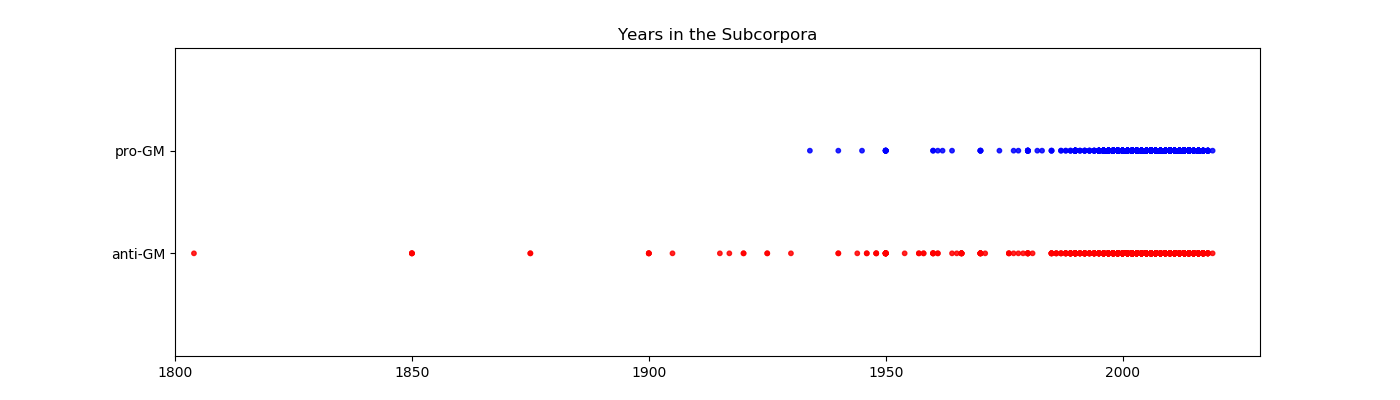
\includegraphics[width=16cm]{Figures/years.png}
\caption{Time horizons in the sub-corpora}
\label{fig:figure1}
\end{figure}

\textbf{Summary of the Cultural-Level}

By themselves, each observation at the cultural level does not lead to any conclusions. Taken together, however, the preceding results suggest that cultural difference is, indeed, a major factor in explaining diverging perspectives between the two sub-corpora. The first indication of cultural divergence is the very use of the term \textit{culture} in the anti-corpus and its relative absence from the pro-corpus. The fact that \textit{culture} appears much more in the anti-corpus and \textit{indigenous} is mentioned nearly 800 times, points to vastly different cultural contexts between the two sub-corpora. 

The geographic entity data suggest the anti-corpus contains a wider range of countries and cities. One could make the case, in turn, that this variety reflects a greater diversity of cultural perspectives. The same could be said for the temporal horizons. The wider span of years in the anti-corpus is suggestive that historical memory and context is at play to a greater degree.

\subsection{Socio-Economic Level}

Divisions in the GM-seed debate are deeply related to socio-economic imbalances and differing conceptions of economic growth. The 1950s and 60s saw the development of Green Revolution technologies (genetically modified/higher yielding crop varieties, synthetic fertilizer and pesticides, irrigation). The development of these technologies was followed by a neo-liberal policy framework in the 1970s and 80s, which (many argue) gave way to consolidation and monopoly control over agricultural supply chains. This included policies in the U.S., Canada and other developed countries that moved seed biotechnology from the public sector to the private seed industry. Vertical integration in agricultural supply chains accompanied horizontal consolidation of intellectual property rights for seed biotechnology. Rapid developments in genetic engineering and biotechnology took place in this economic context, leading to the situation today, where a handful of corporations control the majority of the world's seed markets and patents.

The controversy over GM-seed has coincided with neoliberal economic reforms. Free Trade Agreements (FTAs) have often granted legal intellectual property rights to international seed companies. The prohibition on seed saving can apply not only to patented varieties, but to any seed varieties that have not been registered or pre-approved. As a result, any farmer caught saving and replanting patented or even non-registered indigenous varieties could face fines or even jail time. There have been several cases where these laws led to nation-wide farmer's strikes and protests. For example, in June 2010, tens of thousands of Haitian farmers protested the ``deadly gift'' of seed to the Haitian government. After the devastating earthquake six months prior, smallholder farmers were faced with a shortage of seeds since many rural families used maize seed to feed the masses of refugees. In response, Monsanto (then the world's largest hybrid and GM seed company) announced it had delivered 60 tons of hybrid seeds of maize and vegetables; an additional 400 tons would be delivered throughout the year. Farmers would purchase these seeds from farmer association stores and the store revenue would be re-invested to purchase additional inputs of pesticides and fertilizers. The company itself acknowledged farmers would be unable to save and replant seed. This would potentially make farmers dependent on the market and purchased inputs.

Whether it's the Haiti case or elsewhere, economic analysis suggests that divisions over GM seed are not necessarily a consequence of biotechnology itself, but the economic context in which it has developed. In this for-profit context, purchased seed inputs are developed primarily to meet the circumstances of the largest customers (i.e. farmers with access to large acreages, machinery, credit, and subsidies). Pricing and regulations are established in the same vein. Also, seeking the largest return on investment, market-driven R\&D will naturally emphasize major crop varieties and sales volume, rather than specialty crops and fresh produce that suit local circumstances and small-producers.

The advantages commercial seed offers large-scale farmers do not necessarily translate to small producers and those in the certain parts of the world. For example, the labour-saving potential of GM crops presents a significant financial advantage to a farmer who otherwise would have to target-spray weeds with herbicide. With modern equipment and GM herbicide resistant crops, this farmer could do in hours what previously could take many days of work. The risk of crop failure is offset by insurance as well as government subsidy and income stabilization programs. In this case, planting large acreages with monocrop using commercial seed and chemical inputs, makes sense financially for producers.	

The economic context indicates how commercially patented seed may not fit the economic reality of many of the world's 800 million small-scale food producers. Consequently, those resisting the use of commercial seed varieties might be doing so as part of practical efforts to feed their families and earn a living. In other words, resistance is often based on lived realities faced by small-scale farmers in addition to cultural, ecological, or other factors.

\textbf{Concordances of \textit{Income}}

Here, we explore the hypothesis that economic factors discussed above are reflected in corpus data. The key terms analysis (Table 3.1) suggests that \textit{income} is a much more prominent concept in the pro-GM data. Frequency data further support this view. The word \textit{income} appears in the anti-GM corpus with a frequency of 0.22 per thousand words. In the pro- corpus the frequency is over eight times higher at 1.78. Tables 3.10 and 3.11 below show a sampling of 10 concordances of \textit{income} from both sub-corpora. The collocate \textit{farm income} accounts for the majority (174 of 237) of concordances from the pro-GM corpus. While this same collocate is present in the anti-GM corpus, it appears in only 2 (of 58) concordances.

The contrasting concordances are notable because the term \textit{farm income} is used in national and international policy discourse. In the concordances, the term is used at this higher-level of agricultural policy and economics, often accompanied by statistics spanning the entire sector. It is fair to say the term \textit{farm income} is associated with larger-scale commercial farming. By contrast, in the anti-GM corpus, the term \textit{income} is more likely to occur in the context of smaller-scale, household economics. Collocates \textit{community income}, \textit{household income}, or the possessive \textit{farmers' income} are all more prevalent. The lines refer to income in the context of local produce sales, and subsistence activities. Whereas the pro-GM corpus focuses on income gain and positive impacts, the anti-GM corpus refers more to losses, poverty, and scarcity.

\begin{table}[H]
\begin{footnotesize}
\centering
\begin{tabular}{c} 
\texttt{nology). The additional farm INCOME generated by the technology i} \\
\texttt{s up to 2004. Since then net INCOME gains fell to between \$3/ha a} \\
\texttt{ and \$18/ha. In 2014, the net INCOME gain was \$14/ha. The relative} \\
\texttt{ositive impact on direct farm INCOME in recent years reflects a co} \\
\texttt{997 there has been a net farm INCOME benefit from using the techno} \\
\texttt{f cost of 37 Increase in farm INCOME at a national level (\$ millio} \\
\texttt{tion of impact with yield and INCOME gains widely reported for man} \\
\texttt{rall, in 2014, the total farm INCOME from using the technology was} \\
\texttt{en to about \$20/ha. Net farm INCOME gains (after deduction of the} \\
\texttt{\ \ level is an increase in farm INCOME of \$2.5 million. Cumulatively}
 \end{tabular}
\caption{Concordance lines of \textit{income} Pro-GM corpus}
\label{tab:table1}
\end{footnotesize}
\end{table}

\begin{table}[H]
\begin{footnotesize}
\centering
\begin{tabular}{c} 
\texttt{nd an opportunity to generate INCOME by selling their produce at l} \\
\texttt{ definition of poverty as low INCOME . Poverty can mean the lack o} \\
\texttt{\ orted household and community INCOME generation. Extreme poverty h} \\
\texttt{o produce sufficient food and INCOME from locally-available resour} \\
\texttt{\ egular rather than occasional INCOME generation strategy. After th} \\
\texttt{ies to urban areas, household INCOME and use of non-traditional, p} \\
\texttt{\ \ prices, hurt local farmers' INCOME , and disrupted the usual pat} \\
\texttt{ese two GM crops deliver less INCOME on average to farmers than no} \\
\texttt{d rape sector in Canada; lost INCOME for organic and other GM-free} \\
\texttt{\ ut rather of lack of adequate INCOME to access food. In our countr}
 \end{tabular}
\caption{Concordance lines of \textit{income} Anti-GM corpus}
\label{tab:table1}
\end{footnotesize}
\end{table}

\textbf{Collocates of \textit{Corporate}}

Collocates of the word \textit{corporate} are also a telling indication of economic context in the anti-GM corpus. The corpus was searched for collocates that immediately followed the word \textit{corporate} (1R) and were repeated multiple times (minimum frequency 2). The result is a list with 12 collocations, 11 of which are in the anti-corpus (Table 3.12). These collocates include \textit{corporate control}, \textit{corporate power}, and \textit{corporate greed}. The pro-GM corpus contains only one multi-frequency collocate, \textit{corporate watch}. Many of these collocates are suggestive of an anti-GM discourse that views the topic of GM seed in terms of economic power relations. Some collocates (e.g., \textit{greed}) suggest a critical view of these relations. Other collocates of frequency 1 (not included in 3.12) confirm this critical view. For instance, included in the collocates are corporate \textit{interests}, \textit{lobby}, \textit{secrets}, \textit{evil}, \textit{control}, \textit{domination}, and \textit{shills}.  

The fact that anti-GM discourse is critical of corporate power is not, in itself, surprising. What is worthy to note, however, is that collocates of corporate are comparatively absent from the pro-GM corpus. Insofar as the pro-corpus discusses the topic in economic language, it seems to be in terms of increased efficiency, income, and profit, as reflected in Table 3.10. Economic power relations, it seems, are not discussed.   

\begin{table}[H]
\begin{footnotesize}
\centering
\def\arraystretch{1.1}% 
\begin{tabular}{ | m{2cm} | m{2.25cm} |}  
\hline
\textbf{Frequency} & \textbf{Collocate} \\
\hline
\multicolumn{1}{|c|}{12} & sector \\
\hline
\multicolumn{1}{|c|}{9} & control \\
\hline
\multicolumn{1}{|c|}{4} & seed \\
\hline
\multicolumn{1}{|c|}{4} & power \\
\hline
\multicolumn{1}{|c|}{3} & agriculture \\
\hline
\multicolumn{1}{|c|}{2} & takeover \\ 
\hline
\multicolumn{1}{|c|}{2} & subsidies \\
\hline
\multicolumn{1}{|c|}{2} & pressure \\
\hline
\multicolumn{1}{|c|}{2} & greed \\
\hline
\multicolumn{1}{|c|}{2} & finances \\
\hline
\multicolumn{1}{|c|}{2} & entities \\
\hline
\multicolumn{1}{|c|}{2} & consolidation \\
\hline
\multicolumn{1}{|c|}{2} & concentration \\
\hline
\multicolumn{1}{|c|}{2} & agency \\
\hline
\end{tabular}
\caption{Collocates of \textit{corporate} in the Anti-GM subcorpus}
\label{tab:table1}
\end{footnotesize}
\end{table}

\textbf{Income Split}

The previous analysis of country entities in the corpus suggests that a higher proportion of countries mentioned in the anti-corpus are from the Global South. This result points to possible economic differences between the two sub-corpora. To further explore this hypothesis, GDP data was used. All countries mentioned in the corpus (including city mentions) were ranked according to GDP (nominal) per capita. Among all countries, the average rank, average GDP, and percentages in the top and bottom quartiles (according to GDP), were determined. 

As Table 3.13 shows, all four data points suggest that the anti-GM corpus does indeed reflect lower income countries, though the significance of this difference is debatable. The average country rank (by GDP) is 11 percent lower in the anti-corpus; the average GDP is 8 percent lower; the percentage of countries in the top quartile by GDP is 9 percent lower; and the percentage of countries in the bottom quartile is 19 percent higher than in the pro-GM corpus. 

\begin{table}[H]
\begin{footnotesize}
\centering
\begin{tabular}{|l|l|l|}
\hline
\textbf{}            & \textbf{anti-GM} & \textbf{pro-GM} \\\hline
avg. rank            & 90                      & 81                     \\\hline
avg. GDP             & 20,766                  & 22,370                 \\\hline
\% in top quartile:   & 32                      & 35                     \\\hline
\% in bottom quartile & 38                      & 32                    \\\hline
\end{tabular}
\caption{Income data between the sub-corpora}
\label{tab:table1}
\end{footnotesize}
\end{table}


\textbf{Summary of Socio-Economic Level} 

The GDP statistics, together with the qualitative analysis of concordances of \textit{income}, are evidence that an economic divide exists between the pro and anti sub-corpora. Context of \textit{income} is drastically different between the two sub-corpora. On the one hand, \textit{income} is discussed in the context of profit, efficiency, and financial/capital gain. On the other, \textit{income} is mentioned in the context of subsistence/household economics and even economic hardship. Thus, while the term is central to both sub-corpora, it functions in entirely different contexts. 

The concordances are consistent with the GDP statistics, which give quantitative evidence that the anti-GM corpus is representative of lower income countries and regions. However, the GDP analysis overlooks the extent to which the economic divide might be intra- as well as international. In other words, country GDP data does not capture the extend to which the GM seed debate may be about dominant corporate entities vis-\`a-vis smaller-scale producers within countries.

Finally, the collocates of \textit{corporate} indicate that, not only is there an economic divide between the two sub-corpora, but that the anti-GM discourse is much more engaged in political/economic critique. 


\subsection{Cognitive Level}

The cognitive level aims to understand and compare the mental representations of language users in both sub-corpora. Elements of cognitive analysis of discourse, as outlined by \cite{VanDijk2000a}, include topics, implications, presuppositions, local coherence, and lexical meanings/connotations. Some of these elements have been covered, albeit not explicitly, in the other levels. For example, key word and key term analyses addressed \textit{topics}. Likewise, much of the collocation and concordance discussion relates to \textit{connotations}. 

In addition to elaborating on topics and connotations, this section looks at implication and presupposition. Coherence is examined through the notions of interdiscursivity and conceptual blending. 

\textbf{Implications and Presuppositions}

Implication pertains to cognitive analysis insofar as it contains socially shared knowledge that is inferred from explicit semantic contents of discourse \citep{VanDijk2000a}. Implicature \citep{Grice1975} is inferential and context dependent, that is to say, it relies on knowledge domains or mental schema. \cite{Sperber1995} make the distinction between `implicature' and `explicature', where (in explicature) assumptions are explicity stated. It may be the case that implications are understood more or less universally. It is also possible that implications rely on knowledge that varies across different cultures, communities of practice, or other groups. In such cases, implicature can be a reflection of ``cultural scripts'' \citep{Wierzbicka1985, Wierzbicka2003}.

Discourse is often full of implicature. From a corpus linguistic perspective, the challenge is narrowing the examples in a way that is consistent and comparable. Of course, identifying implicit assumptions by computationally searching a corpus is also a challenge.  In order to get a representative sample of implications in the corpus, we can look at collocates of the word \textit{means}, which is a common way to express implication in spoken and written English (i.e. A \textit{means} B). Although this relationship between A and B may be explicit, the assumptions underlying this relationship may not be.   

There are 81 and 43 such collocates in the anti- and pro-GM sub-corpora, respectively. The lines were manually and qualitatively analyzed and written in symbolic notation with a right arrow ($\rightarrow$) used to signify implication between propositions (e.g., A $\rightarrow$ B $\rightarrow$ C). The numbered segments below contain selected examples of implications in the pro-GM subcorpus, together with summarized implication relationships (in bold).

\begin{footnotesize}
\begin{quote}
\begin{enumerate}

  \item \texttt{Easier farming MEANS more food which, in turn, MEANS less expensive food.} \textbf{[Easier farming $\rightarrow$ more food $\rightarrow$ cheaper food]}\\

   \item \texttt{Decreased use of pesticides, MEANS less pesticide production demand and also less energy use on the farmers' end, too.}\\ \textbf{[Decreased pesticide use $\rightarrow$ less energy use]}\\
   
   \item  \texttt{Many plants are designed to use less pesticides and chemicals to grow, which MEANS less exposure to these potentially toxic substances for farmers and consumers.}\\ \textbf{[Less pesticides $\rightarrow$ less exposure to toxins]}\\
   
   \item  \texttt{Many GMOs are tailored for specific environmental conditions, which MEANS saving water in drought-prone areas and less use of chemicals.}\\ \textbf{[GMO seed $\rightarrow$ saving water AND less chemical use]}\\
   
   \item  \texttt{...GM [foods] have improved flavor and texture, as well as delayed ripening. This MEANS produce will stay fresh for longer periods of time.}\\ \textbf{[GMO seed $\rightarrow$ delayed ripening $\rightarrow$ produce stays fresh longer]}
  
\end{enumerate}
\end{quote}
\end{footnotesize}

The five examples above express relationships among different variables, such as food supply and food prices (1); pesticide use and energy use (2); pesticide use and toxins (3); genetic modification and water/chemical use (4); and genetic modification and preservation of freshness (5). Of interest, is the extent to which these relationships are explicit and quantifiable. Moreover, the logic of the relationships is more-or-less self explanatory as, for instance, the relation between food supply and food prices. In fact, in each example, the reader could conceive of a mathematical function depicting the relationship in question. Moreover, this relationship is often two dimensional; that is, between two variables (e.g. seed type and preservation time). Overall, little additional context is necessary to explain the relationships in question. Now, consider some examples from the anti-GM corpus:

\begin{footnotesize}
\begin{quote}
\begin{enumerate}

  \item \texttt{farmers...quickly lose control over seed management, production and eventually their land. This MEANS they lose their food sovereignty...} \textbf{[GM seed $\rightarrow$ loss of control over seed management $\rightarrow$ loss of food sovereignty}\\
  
  \item \texttt{...Monsanto (and other companies) own the rights to the modified DNA in their seeds. This MEANS farmers would have to buy seeds from them each year, and maybe more than once.} \textbf{[companies own seed rights $\rightarrow$ farmers have to buy seed annually]}\\
  
  \item \texttt{...they will cause reduced genetic diversity of plants and animals in the environment. What this MEANS is that the DNA, which codes for proteins in an organism, will become more similar between individuals of a species.} \textbf{[ reduced genetic diversity $\rightarrow$  loss of biodiversity]}\\
  
  \item \texttt{And if Paraguay is so dependent [on foreign companies] for such a basic thing as food...it MEANS that this is a subordinate country.} \textbf{[food dependence $\rightarrow$ national subordination ]}\\
  
  \item \texttt{...the nature of the promoter MEANS that the inserted genes are liable to be unstable and move out again.} \textbf{[promoter genes $\rightarrow$ instability in inserted genes $\rightarrow$ plant instability and variable gene functioning $\rightarrow$ unintended effects]}\\
  
  \item \texttt{...just three companies sell more than half the seeds on the market...this MEANS that the biological diversity of crops is declining, making our food supply less likely to adapt well to climate change.} \textbf{[three companies control seed market $\rightarrow$ declining biodiversity $\rightarrow$ less adaptive food supply]}\\
  
\end{enumerate}
\end{quote}
\end{footnotesize}

In comparison with the pro- examples, the implications above are not quantifiable. In many, cases the propositions cannot be expressed as variables; rather, the relationships involve implicit contextual or subjective factors that often evade objective representation. Consider the following relationships: GM seed and food sovereignty (1); food dependence and national subordination (4); and, biodiversity and adaptability of the food supply (6). In these cases, the relationship would be very difficult (if not impossible) to quantify. Moreover, an understanding of these relationships demands context based on an implicit set of factors/assumptions. 1 and 3, for example, invoke cascading sets of political/economic consequences induced by the adoption of GM seed by farmers, and culminating in loss of national sovereignty.     

In other cases, the relationships invoke biological complexity. In 5, the antecedent proposition (\textit{promoter gene}) leads to \textit{unintended consequences} via genetic instability. Similarly, in 6 the connection between seed market concentration, biological diversity, and ability to adapt to climate change depends on a complex set of factors.

Together, the implications observed in the corpus reinforce what is observed in the ecological level of analysis. Compared to the pro-subcorpus, the anti-GM discourse rests on mental models characterized by complex systems and conceptual schema that aims to encompass interrelations among multiple factors. Pro-GM discourse, by contrast, tends towards quantifiable relationships. 

\textbf{Interdiscursivity and Conceptual Blending}

The claim that anti-GM discourse operates in the context of more ``complex systems,'' is not meant to imply it is somehow more truthful or accurate. Rather, it is an attempt to characterize the conceptual and mental space within which the discourse operates. It is suggested that interactants in anti-GM discourse construct meaning by combining and mapping concepts from different mental spaces in ways that are not common in pro-GM discourse. Blending Theory \citep{Turner2002}, tells us that this combining and mapping of concepts gives rise to meaning as an emergent structure that is beyond the sum of its parts \citep[403]{Evans2006a}. While pro-GM discourse evidently employs conceptual blending in its own right, the results of preceding sections suggest that the emergent structure of the anti-GM discourse differs in the size and number of input spaces that contribute to an emergent structure of meaning. 

To pursue the basic idea that concepts are combined to form emergent meaning, we can consider interdiscourse as a particular manifestation of Blending Theory. Interdiscourse refers to the relations that a discourse has to other discourses. Drawing from \citep{Bullo2017a}, we propose that interdiscourse is part of a process of conceptual integration and sense making. As an example, we examine an excerpt from the anti-GM subcorpus. The following excerpt is from the ``Maize Manifesto'' released January 15, 2013 by the National Union of Autonomous Regional Peasant Organizations (UNORCA) in Mexico.

\begin{footnotesize}
\begin{quote}
\texttt{\justify In our country there are more than 60 native races and thousands of local varieties of maize, which instead of representing some kind of risk, carry important virtues thanks to their selection and adaptation by indigenous peoples over more than seven thousand years. Some of these native varieties offer higher yields than the ones manipulated by Monsanto. The imposition of transnational frankenseeds would mean an end to this richness and the loss of the ancestral milpa tradition as a sustainable system of maize production and symbol of the Mesoamerican cultural inheritance.}
\end{quote}
\end{footnotesize}

A high degree of interdiscursivity appears in this text. In this excerpt (and the Manifesto as a whole) the scientific discourse is not dismissed, but hedged as ``some kind of risk'' suggesting that, despite empirical research, there are unknowns associated with the technology. Scientific and technical aspects are explicitly acknowledged in this way, but are also implicitly placed in the framework of ancestral tradition and culture. Transitivity suggests interconnectedness and blurred boundaries between nature and culture. The notion of ``selection and adaptation'' of seed varieties over thousands of years suggests a natural attunement to complex biological processes, in contrast to an unnatural, hubristic ``manipulation'' of varieties by a large corporation. Similarly, the colonial, historical images could also work as a biological metaphor. The age-old Mayan milpa tradition of crop rotation and nutrient cycling being lost at the hands of a ``transnational'' seed is akin to an invasive species threatening an ecosystem. The historical context is also referred to in the use of the geographic term ``Mesoamerica'' (a cultural and bioregion) as opposed to the more historically recent nation states of the region. 

\textit{Frankenseeds} is itself an example of a type of conceptual blending known as compounding, whereby two or more morphemes combine to form a word \citep[415]{Evans2006a}. A subset of the meanings associated with each morpheme combines to give a unique and distinct meaning. The term \textit{frankenseeds} appears in both sub-corpora and is used among GM critics. Of course, the word invokes Shelly's Frankenstein, which is a portrayal of the dark side of industry and science as well as romanticism as a reaction to industrialization and Enlightenment disenchantment. Putting these literary themes in the context of GM seed is merely one example of how complex blending of concepts occurs in the excerpt and in GM discourse as a whole (Figure 3.2). 

To summarize, this excerpt demonstrates interconnectedness and layers of rich meaning that combine to form an emergent meaning that blends scientific worldviews, culture, nature, and history. 

\begin{figure}[H]
\centering
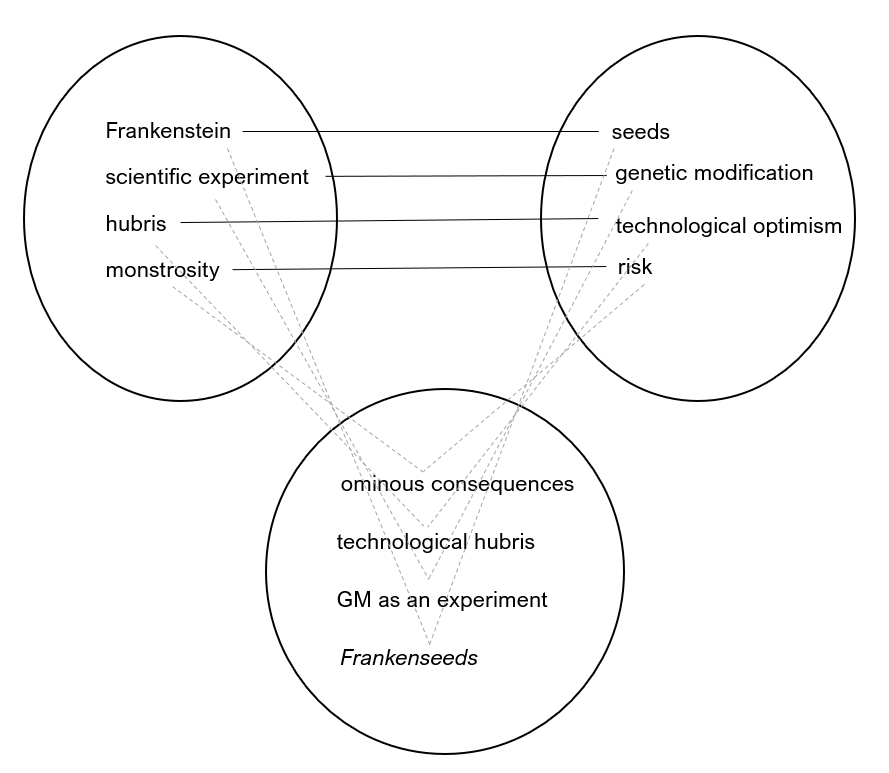
\includegraphics[width=8cm]{Figures/blending.png}
\caption{Compound blending to form \textit{Frankenseeds}}
\label{fig:figure1}
\end{figure}

\textbf{Situated Context}

In addition to blending of concepts within the corpus, we can also consider how non-discursive practices relate to the text. Such considerations are crucial at the cognitive level in light of situated cognition, or the premise that knowledge is inseparable from action. In other words, knowledge (and therefore discourse) is bound to social, cultural, and physical contexts \citep{Greeno1998}. The ``Maize Manifesto'' is not merely an article; rather, it is an political act that accompanied protests and hunger strikes by indigenous peasants in the Mexican capital. In short, the text is not understood in isolation, but in the situated context within which it was produced. 

The ``Maize Manifesto'' passage, together with results from the earlier section \textit{Specialization and Communities of Practice}, points to possible differences in extra-linguistic context between the sub-corpora. Specifically, we can consider that the anti-GM discourse takes place in the context closer to situated engagement with the topic, whereas as the pro- discourse is more likely to approach the topic through a third person, objective observer. Theoretical and empirical/scientific claims of pro-GM discourse contrast with the first-person lifeworld perspective of certain actors, such as those who produced the ``Maize Manifesto'' text. 

The essence of GM seed is often framed as a biological object. This is the logical result of a conceptual approach that presupposes a human as subject and the genetically altered organism as object. As such, discursive truth claims ultimately rest with those who possess specialized knowledge of this object relation (i.e. molecular biologists); those who take a third-person position over and against the object of study. In contrast, speakers in the ``Maize Manifesto'' begin with human experience and confront how GM technology is embedded in a plurality of contexts. 

\section{Summary \& Conclusions}

This chapter began by pointing out the complex nature of the GM seed debate. Through a multi-level analysis, the topic was broken down in order to view it from various perspectives. By splitting the corpus into two distinct sub-corpora, it was possible to gain insights into sources of misunderstanding and disagreement between sides of the debate. The following is a summary of findings:

\begin{itemize}
  \item Pro-GM discourse is significantly more likely to come from corporate or for-profit entities, while the anti-GM discourse is more likely to originate from non-profit or advocacy organizations. 
  \item Anti-GM discourse contains culturally significant key words and key phrases while those in the pro-GM discourse are more technical and specialized. 
  \item Concordance analysis also suggested \textit{culture} is a far more prominent factor in the anti-GM discourse.
  \item Anti-GM discourse is more likely to view natural systems holistically whereas the pro-GM discourse takes a more analytic and reductionist approach.
  \item The countries mentioned in the corpus are more distributed in the anti-GM subcorpus.
  \item Based on years and decades mentioned, the temporal span in the anti-GM corpus is larger.
  \item Concordances of \textit{income} suggest the economic context in the sub-corpora is different, with the anti-subcorpus focused more on economic scarcity and household income as opposed to the term \textit{farm income} in the pro-subcorpus.
  \item Based on collocates of \textit{corporate}, the anti-GM discourse is more critical of socio-economic structures.
  \item Analysis of the country data suggests that lower income countries are more represented in the anti-GM corpus.
  \item Analysis of implications suggests the pro-GM subcorpus explains relationships in more quantifiable variables, whereas the anti-subcorpus contains more qualitative, subjective, and unquantifiable relationships.
  \item Interdiscursivity, conceptual blending, and situated context all seem to be markedly different between the two sub-corpora.
\end{itemize}

Before drawing any conclusions from these findings it is important to point out an underlying assumption; namely, that the corpus is representative of GM seed discourse. Assuming the corpus does, to a significant extent, represent the societal discourse on the topic, the multi-level results are significant. Taken alone, each of the above results is not telling. However, taken together, the above findings point to crucial differences between the two sub-corpora and, hence, between the two sides of the GM seed debate.

The results suggest that the anti-GM discourse embodies a plurality of actors in a way that the pro-GM discourse does not. This plurality is suggested in the distribution of countries/geographic entities in the corpus as well as the cultural context of the anti-GM subcorpus. In addition, the cognitive analysis indicates that intersubjectivity, or psychological connotations/first-hand experiences with respect to GM seed, is an undercurrent in the anti-GM discourse. Intersubjectivity is itself an expression of plurality, insofar as it is the coming together of diverse human subjects. This intersubjective orientation is in contrast to the third-person, subject-object perspective pro-GM discourse. 

The plurality inherent in anti-GM discourse points to a possible source of misunderstanding between different sides of the debate. In the face of the complex web of relationships and perspectives, people may attempt to organize and categorize the discourse into familiar categories and frames. Cognitively, this categorization functions similar to stereotype, where information is simplified in order to make sense of an otherwise too complex world \citep{Tajfel1981}. No doubt, this simplification is inevitable in the face of a complex topic such as GM seed. However, the condition of plurality in the anti-GM discourse makes this side of the debate particularly susceptible to reduction and simplification on the part of their critics.

In order to see this simplification at play in GM seed debate, consider the following excerpt from the pro-GM subcorpus. The excerpt is from the article ``The Truth about Genetically Modified Food'' by David H. Freedman in the August, 2013 issue of the magazine \textit{Scientific American}. 

\begin{footnotesize}
\begin{quote}
\texttt{\justify Some scientists say the objections to GM food stem from politics rather than science\textemdash that they are motivated by an objection to large multinational corporations having enormous influence over the food supply; invoking risks from genetic modification just provides a convenient way of whipping up the masses against industrial agriculture. "This has nothing to do with science," Goldberg says. "It's about ideology." Former anti-GM activist Lynas agrees.  He recently went as far as labeling the anti-GM crowd "explicitly an antiscience movement."}\\

\texttt{It is also true that many pro-GM scientists in the field are unduly harsh\textemdash even unscientific\textemdash in their treatment of critics. GM proponents sometimes lump every scientist who raises safety questions together with activists and discredited researchers.... Most of them are nonscientists, or retired researchers from obscure institutions, or nonbiologist scientists....}
\end{quote}
\end{footnotesize}

The dominant frame in this text is that of empirical science, specifically peer reviewed research in a setting of certain prestige Anglo-American institutions. Alternate social and institutional meanings are secondary, if at all considered. The article as a whole does raise the concern of perceived influence of industry funding on research perspectives. Also, possible unknowns inherent in the scientific research are pointed out. However, there is an ordering of discourses below the scientific. In an apparent representation of both sides of the debate, the possible flawed (``unduly harsh\textemdash even unscientific'') position of some GM proponents is not a result of their failure to consider alternate discourses, but that they ``lump'' otherwise objective scientific concerns together with non-scientific perspectives of ``activists and discredited researchers.'' In other words, the pro-GM argument would be even stronger if they ignored non-scientific discourses all together. These non-scientific perspectives include those related to politics, corporate influence, industrial agriculture; those advanced by activists, nonbiologist scientists, or researchers at ``obscure institutions.'' Identity construction and word choice (``masses,'' ``crowd,'' ``activists,'' ``obscure,'' ``retired,'' ``ideology,'' ``discredited'') are used pejoratively in contrast to seven instances where ''science'' has an unreservedly positive connotation.

The excerpt above is an example of how the plurality of perspectives of GM critics is framed in a simplified manner. In fact, in this excerpt the other side of the debate is characterized maintaining the same frame as was used to reinforce the pro-GM perspective. From the multi-level analysis we see that the pro-GM discourse is more focused on empirical science, analysis, and reduction of complex systems. In the excerpt, these same methods are used to characterize/critique the other side of the debate. However, the multi-level analysis suggests that an understanding of the anti-GM discourse requires entirely different modes of understanding. The anti-GM discourse is based on epistemological as well as cultural, political-economic, and even cognitive factors, the understanding of which requires consideration of multiple-levels and perspectives. Approaching the debate without full consideration of its multi-level nature inevitably leads to misunderstanding. 